
                \begin{figure}
                    \centering
                    \begin{tikzpicture}
                        \pgfplotsset{%
                            width=1\textwidth,
                            height=0.4\textheight
                        }
                        \begin{axis}[
                            xlabel={Runs since restart},
                            ylabel={Average dynamic energy (watt)},
                            ymin=0,ymax=70,
                        ]
                        
                            \addplot [mark=none, densely dashed, red]  coordinates {
                            (1, 19.73790788402818)(2, 18.081814688529462)(3, 27.898987121823808)(4, 17.84392707638979)(5, 17.71410661329038)
                            };
                            \addlegendentry{workstation - IntelPowerGadget}
                            
                            \addplot [mark=none, densely dashed, blue]  coordinates {
                            (1, 19.183969713798245)(2, 18.048697213767806)(3, 18.10548096477223)(4, 17.969210775235464)(5, 17.636008024440272)
                            };
                            \addlegendentry{workstation - HardwareMonitor}
                            
                        \end{axis}
                    \end{tikzpicture} 
                \caption{A graph illustrating the energy consumption of Cores for test case Nbody with regards to how long ago the DUT was restarted (with outliers)} \label{fig:Nbody_Cores_iteration_exp2}
                \end{figure}
                